%\documentclass[notes, t]{beamer}       % print frame + notes
% \documentclass[notes=only]{beamer}   % only notes
% \documentclass[t, aspectratio=169, notes]{beamer}              % only frames
\documentclass[t, aspectratio=169]{beamer}    

\usepackage{color,xcolor}
\usetheme{TUD} % Beamer theme v 3.0
%\setbeamertemplate{note page}[plain]

\usepackage{tikz}
\usetikzlibrary{positioning,chains,arrows,shadows,fadings,shapes,backgrounds,snakes,matrix,patterns,plotmarks,trees,mindmap, calc}
\usepackage{pgfpages} 
\setbeamertemplate{note page}[plain]
\usepackage{pgfplots}
\pgfplotsset{compat = 1.3}
\usepackage{amsmath}% http://ctan.org/pkg/amsmath
\usepackage{kbordermatrix}% http://www.hss.caltech.edu/~kcb/TeX/kbordermatrix.sty
%\usepackage[demo]{graphics}

%\setbeameroption{show notes on second screen=right}

\usepackage{caption}
\captionsetup{font=footnotesize}

\definecolor{1F77B4}{HTML}{1F77B4}
\definecolor{FF7F0E}{HTML}{FF7F0E}
\definecolor{2CA02C}{HTML}{2CA02C}
\definecolor{D62728}{HTML}{D62728}
\definecolor{9467BD}{HTML}{9467BD}
\definecolor{8C564B}{HTML}{8C564B}
\definecolor{E377C2}{HTML}{E377C2}
\definecolor{7F7F7F}{HTML}{7F7F7F}
\definecolor{BCBD22}{HTML}{BCBD22}
\definecolor{17BECF}{HTML}{17BECF}

\let\marvosymLightning\Lightning
\usetikzlibrary{calc}

\usepackage{etoolbox,refcount}
\usepackage{multicol}
\usepackage{mathtools}

\newcounter{countitems}
\newcounter{nextitemizecount}
\newcommand{\setupcountitems}{%
	\stepcounter{nextitemizecount}%
	\setcounter{countitems}{0}%
	\preto\item{\stepcounter{countitems}}%
}
\makeatletter
\newcommand{\computecountitems}{%
	\edef\@currentlabel{\number\c@countitems}%
	\label{countitems@\number\numexpr\value{nextitemizecount}-1\relax}%
}
\newcommand{\nextitemizecount}{%
	\getrefnumber{countitems@\number\c@nextitemizecount}%
}
\newcommand{\previtemizecount}{%
	\getrefnumber{countitems@\number\numexpr\value{nextitemizecount}-1\relax}%
}
\makeatother    
\newenvironment{AutoMultiColItemize}{%
	\ifnumcomp{\nextitemizecount}{>}{3}{\begin{multicols}{2}}{}%
		\setupcountitems\begin{itemize}}%
		{\end{itemize}%
		\unskip\computecountitems\ifnumcomp{\previtemizecount}{>}{3}{\end{multicols}}{}}
		
\newcommand\irregularcircle[2]{% radius, irregularity
  \pgfextra {\pgfmathsetmacro\len{(#1)+rand*(#2)}}
  +(0:\len pt)
  \foreach \a in {10,20,...,350}{
    \pgfextra {\pgfmathsetmacro\len{(#1)+rand*(#2)}}
    -- +(\a:\len pt)
  } -- cycle
}

\usepackage{algorithm2e}
\usepackage{algorithmic}
% \usepackage{algorithm}
% \usepackage[noend]{algpseudocode}
% \usepackage[linesnumbered,ruled,vlined]{algorithm2e}
% \SetKwInput{KwInput}{Input}                % Set the Input
% \SetKwInput{KwOutput}{Output}              % set the Output   

%\usepackage[latin1]{inputenc}
%\usepackage[TS1,T1]{fontenc}
\usepackage{array}
\usepackage{lipsum}
\usepackage{wasysym}

\usepackage{graphicx}
\usepackage{wrapfig}
\usepackage{subfig}
\usepackage{placeins}

\usepackage[
colorlinks=true,
urlcolor=blue,
linkcolor=green
]{hyperref}

\usepackage{subcaption}

%\usenavigationsymbols

\graphicspath{{../../cfigures/}{./}{figs/}{figures/}{../logos/}{../cfigures/}{../RTS-2011/figs/}{fig/}{}}

\usepackage[absolute,overlay]{textpos}

%\newcommand{\floor}[1]{\left\lfloor{#1}\right\rfloor}
\newcommand{\setof}[1]{\left\{{#1}\right\}}
\newcommand{\set}[2]{\left\{{#1}\mid{#2}\right\}}
\newcommand{\ceiling}[1]{\left\lceil{#1}\right\rceil}
\newcommand{\red}[1]{\textcolor{red}{#1}}
\newcommand{\blue}[1]{\textcolor{blue}{#1}}
\newcommand{\yellow}[1]{\textcolor{yellow}{#1}}
\newcommand{\green}[1]{\textcolor{green}{#1}}
\newcommand{\orange}[1]{\textcolor{orange}{#1}}

\newcommand{\suml}[2]{
  \sum\limits_{#1}^{#2}
}

\newcommand{\ceil}[1]{
  \left\lceil #1 \right\rceil
}

\newcommand{\floor}[1]{
  \left\lfloor #1 \right\rfloor
}

\newenvironment{mynamedtheorem}[1]
{\begin{beamerboxesrounded}[upper=uppertheoremcol,lower=lowertheoremcol,shadow=true]{Theorem
#1}} {\end{beamerboxesrounded}}

\tikzset{
	task/.style={shade, shading=radial, rectangle,minimum height=.08cm,
		inner color=#1!60, outer color=#1!60},
	%task1/.style={task=yellow, minimum width=8mm},
	task1/.style={task=blue, minimum width=8mm},
	task2/.style={task=orange, minimum width=13mm},
	task3/.style={task=red, minimum width=13mm},
	task4/.style={task=green, minimum width=13mm},
	task5/.style={task=yellow, minimum width=13mm},
	task6/.style={task=purple, minimum width=13mm},
	task7/.style={task=cyan, minimum width=13mm},
	task8/.style={task=pink, minimum width=13mm},
	task9/.style={task=white, minimum width=1mm, inner color=white, outer
		color=white},
	task0/.style={rectangle, task=gray, minimum width=1mm}
}

\tikzstyle{circleNode}=[circle,thick,draw=blue!75,fill=blue!20,minimum size=6mm]
\tikzstyle{niceFill}=[thick,draw=blue!75,fill=blue!20,minimum size=6mm]


\begin{document}

\title[]{3D Scanning und automatische
Neupositionierung von 3D Modellen}
%\subtitle{Automated 3D scan based CAD-repositioning for design and verification in one-off construction\\by\\Stephan Mönchinger, RobertSchröder, RainerStark}
\author[Niklas Thieme]{\small \underline{}}
\institute[TU Dortmund]{\small Niklas Thieme Proseminar\\
	TU Dortmund University, Germany
}
\date{\today}
\begin{frame}[plain]
  \maketitle
  \vspace{1.5cm}  
  %{\scriptsize This research is supported in parts by the German Research Foundation (DFG) as part of SFB876 and SPP1500.}
\end{frame}

%

\begin{frame}{3D Scan und Positionierung}
    \begin{minipage}[b]{.49\textwidth}
    \begin{block}{Gliederung}
        \begin{itemize}
            \item 3D Druck
            \item 3D Modell
            \item Photogrammetrie
            \begin{itemize}
                \item 3D Scanning
                \item Verfahren
                \item Alternativen
            \end{itemize}
            \item CAD-Neupositionierung
            \begin{itemize}
                \item Einsatzweck und Idee
                \item Verfahren
            \end{itemize}
            \item Zusammenfassung
        \end{itemize}
        \end{block}
        \end{minipage}
        \begin{minipage}[b]{.49\textwidth}
        \begin{figure}
            \centering
            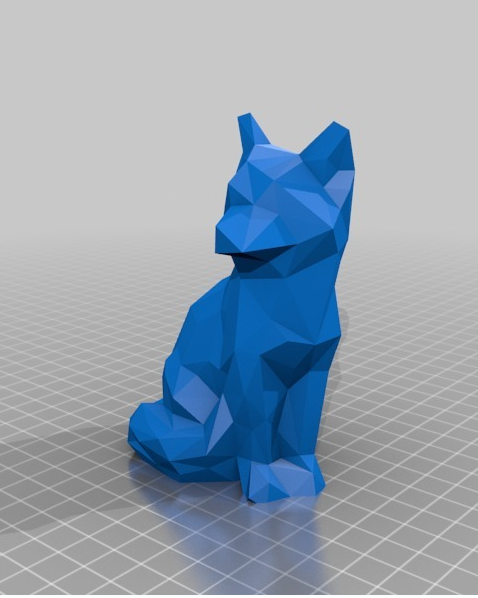
\includegraphics[width=130pt]{img_niklas/fox.PNG}
            \label{fig:my_label}
        \end{figure}
        \end{minipage}

\end{frame}

\begin{frame}{3D Druck}
    \begin{minipage}[b]{.6\textwidth}
    \begin{figure}
        \centering
        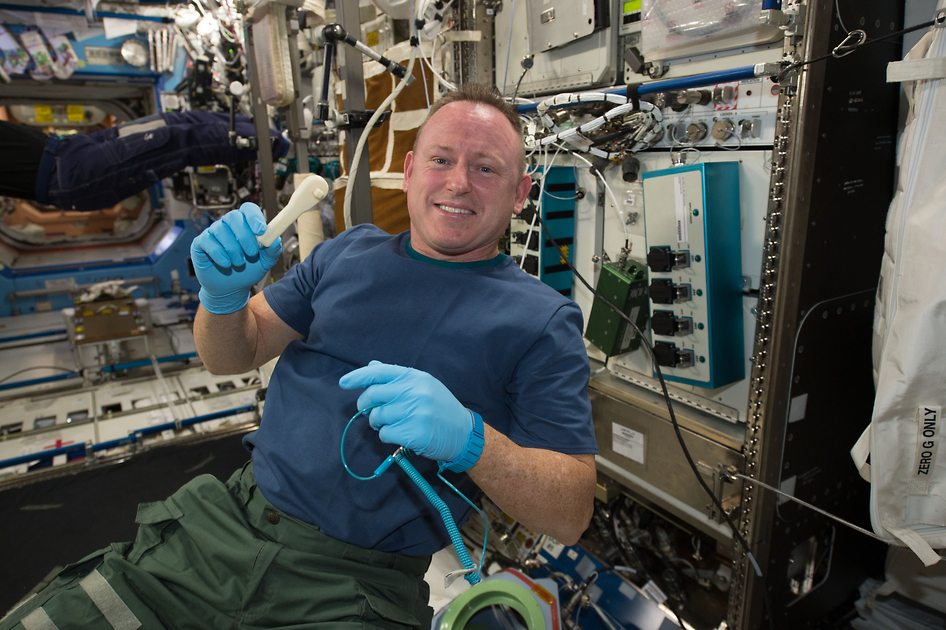
\includegraphics[width=190pt]{img_niklas/iss_wrench.jpg}
        \caption*{ISS Schraubenschlüssel}
        \label{fig:my_label}
    \end{figure}
    \end{minipage}
    \hfill
    \begin{minipage}[b]{.39\textwidth}
    \begin{block}{3D Drucker}
        \begin{itemize}
            \item Einsatzwecke
            \begin{itemize}
                \item Industrie
                \item Heimnutzung
                \item Forschung
            \end{itemize}
            \item Verschiedene Typen
            \begin{itemize}
                \item Ähnliche Arbeitsweisen
                \item Verschiedene Anforderungen
            \end{itemize}
            \item Funktionsweise
            \item Dateiformat STL
        \end{itemize}
    \end{block}
    \end{minipage}
    
\end{frame}

\begin{frame}{3D Drucker Typen}
    \begin{figure}[t]
        \centering
        \begin{minipage}[m]{0.49\textwidth}
        \begin{figure}
            \centering
            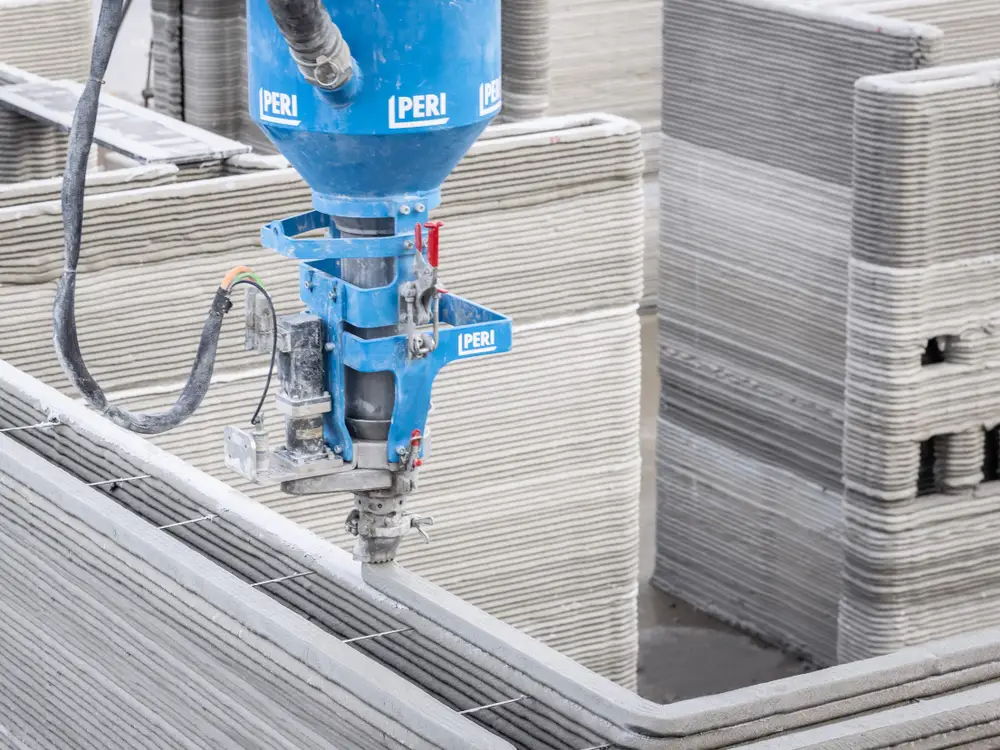
\includegraphics[height=90pt]{img_niklas/3dhouse.png}
            \label{fig:my_label}
        \end{figure}
        \end{minipage}
        \begin{minipage}[m]{0.49\textwidth}
         \begin{figure}
            \centering
            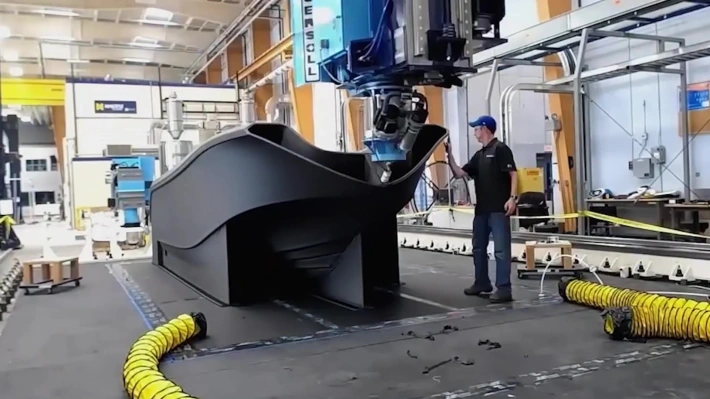
\includegraphics[height=90pt]{img_niklas/3dboat.png}
            \label{fig:my_label}
        \end{figure}
        \end{minipage}
    \end{figure}
    %%bottom
     \begin{figure}[b]
        \centering
        \begin{minipage}[m]{0.49\textwidth}
        \begin{figure}
            \centering
            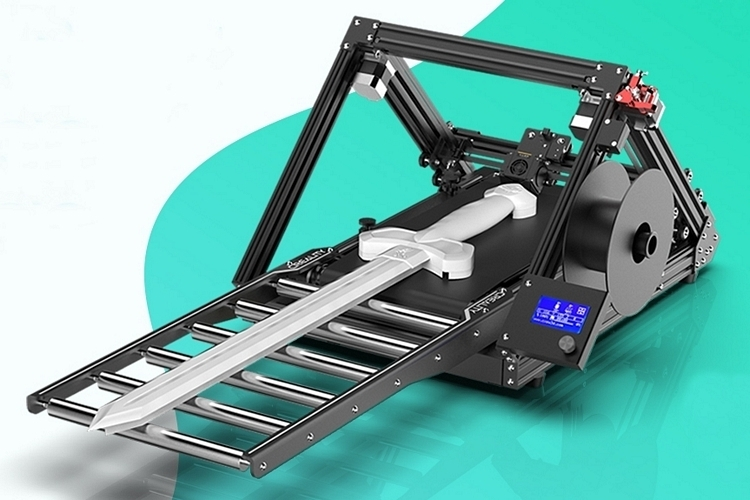
\includegraphics[height=90pt]{img_niklas/creality-cr30-3dprintmill-1.jpg}
            \label{fig:my_label}
        \end{figure}
        \end{minipage}
        \begin{minipage}[m]{0.49\textwidth}
         \begin{figure}
            \centering
            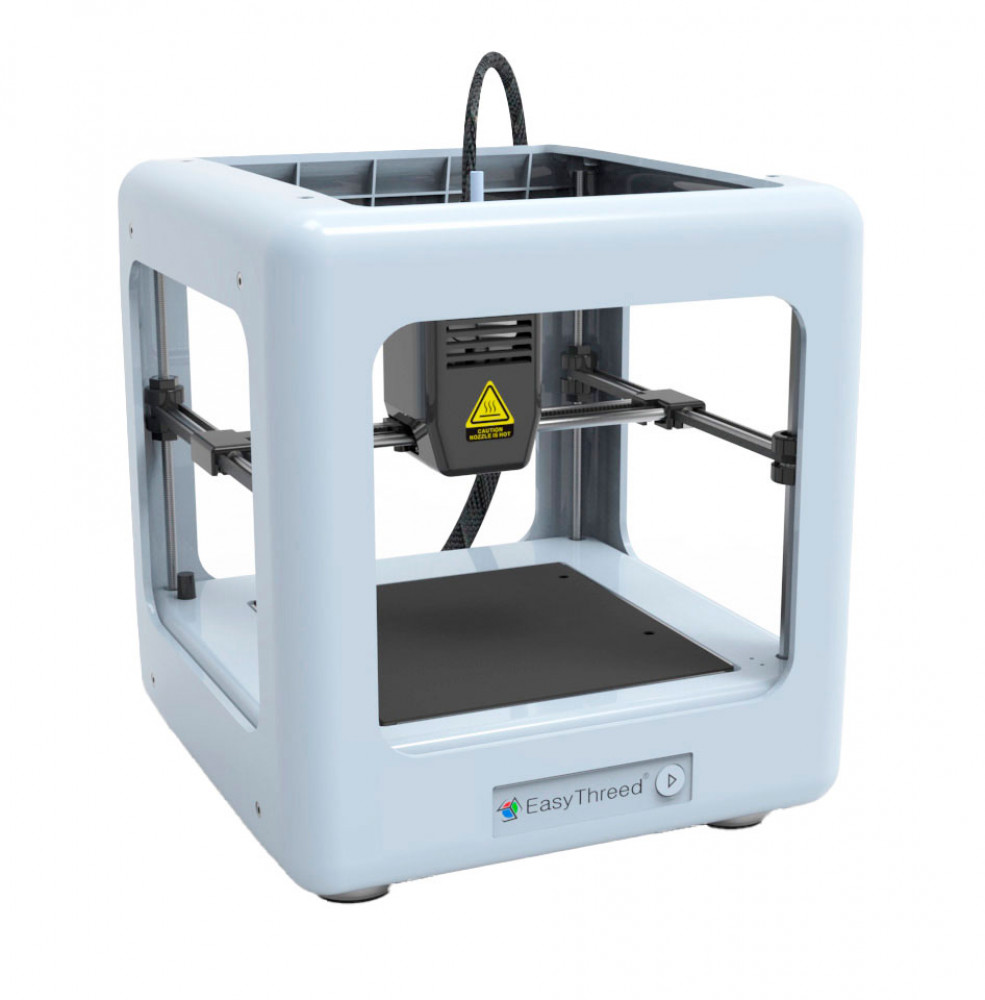
\includegraphics[height=90pt]{img_niklas/3d_printer2.jpg}
            \label{fig:my_label}
        \end{figure}
        \end{minipage}
    \end{figure}
    
\end{frame}

\begin{frame}{FDM vs SLA}
    \begin{minipage}[b]{.45\textwidth}
    \begin{figure}
        \centering
    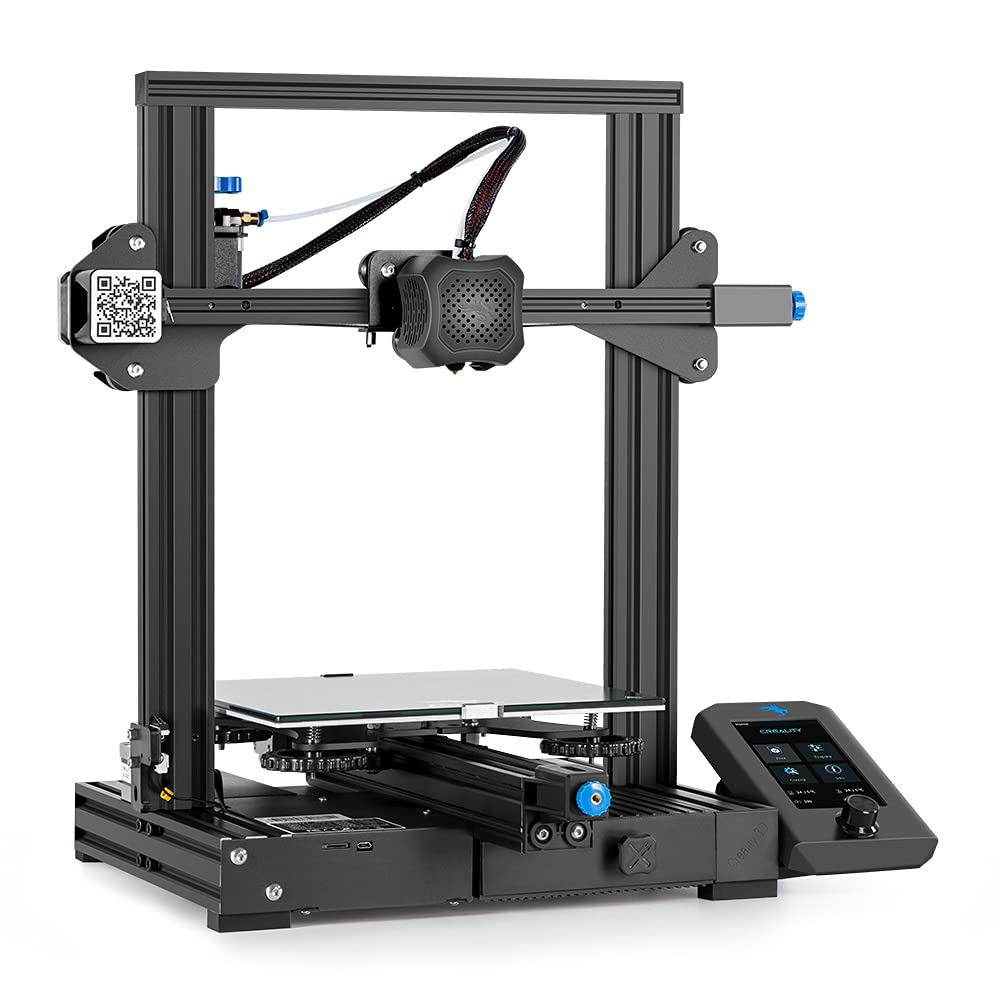
\includegraphics[width=150pt]{img_niklas/3d_printer.jpg}        
    \caption*{Fused Deposition Modeling (FDM)}
    \end{figure}
    \end{minipage}
    \begin{minipage}[b]{.45\textwidth}
    \begin{figure}[]
        \centering
        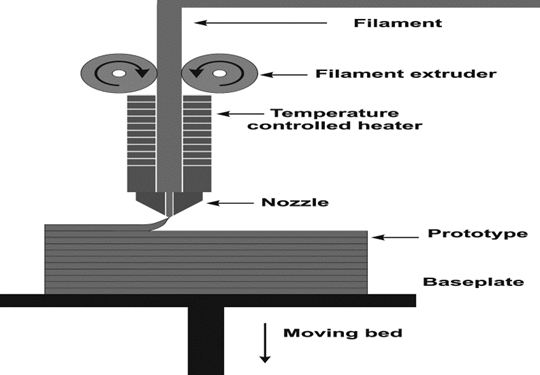
\includegraphics[width=150pt]{img_niklas/Schematic-of-an-FDM-3D-printer-Reproduced-with-permission-from-12.png}
        \caption*{FDM Funktionsweise}
        \label{fig:my_label}
    \end{figure}
    \end{minipage}
\end{frame}

\begin{frame}{FDM vs SLA}
    \begin{minipage}[b]{.45\textwidth}
    \begin{figure}
        \centering
        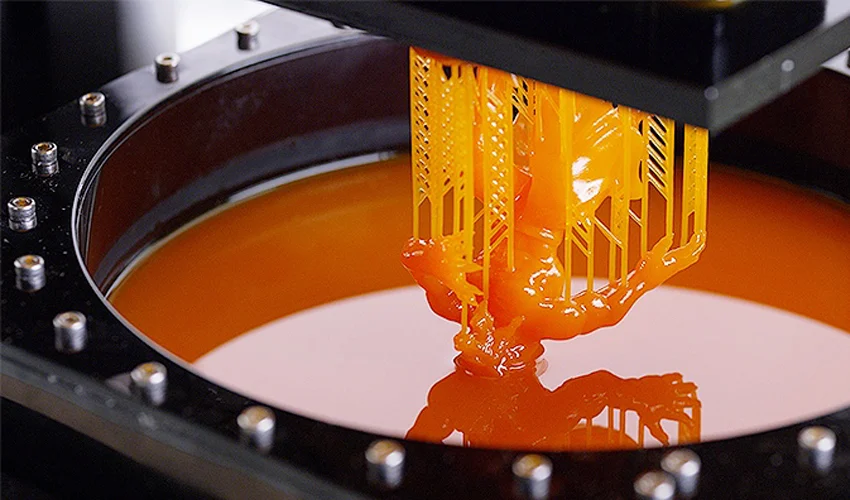
\includegraphics[width=150pt]{img_niklas/SLA_Technology-1.png}
        \caption*{Stereolithografie (SLA)}
        \label{fig:my_label}
    \end{figure}
    \end{minipage}
    \hfill
    \begin{minipage}[b]{.45\textwidth}
    \begin{figure}[]
        \centering
        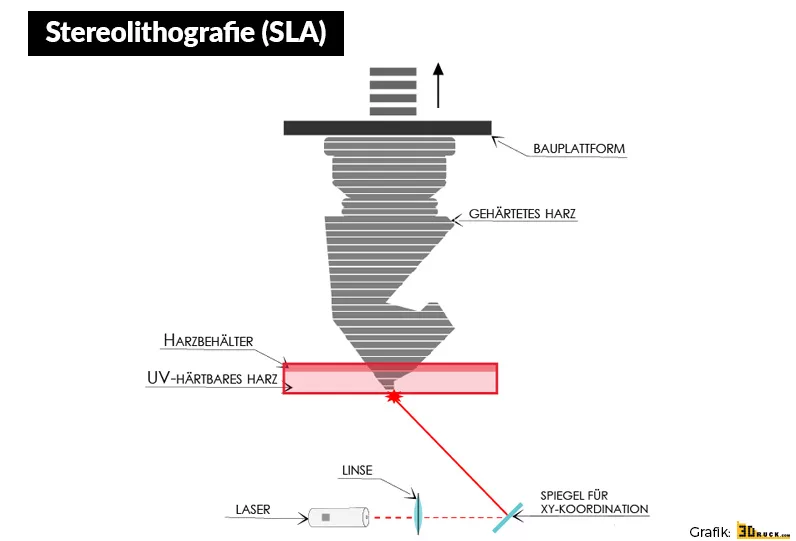
\includegraphics[width=180pt]{img_niklas/sla-stereolithografie-3d-druck.jpg.png}
        \caption*{SLA Funktionsweise}
        \label{fig:my_label}
    \end{figure}
    \end{minipage}
\end{frame}

\begin{frame}{Dateiformat STL}
    \centering
    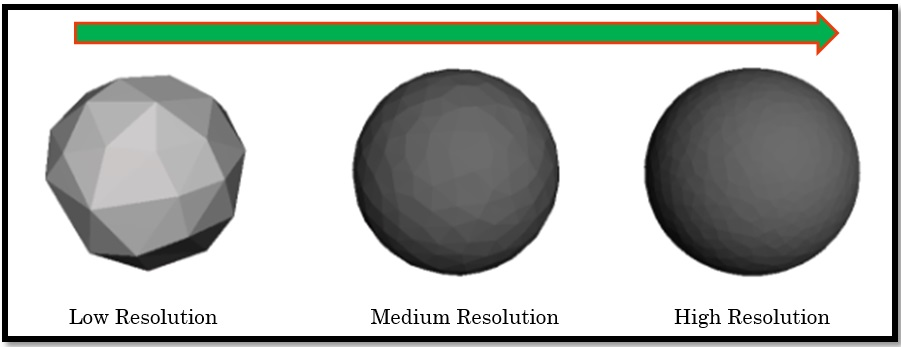
\includegraphics[width=300pt]{img_niklas/stl.jpg}
    \begin{figure}
        \centering
        \begin{minipage}[m]{0.3\textwidth}
        \begin{itemize}
            \item Standard Transformation Language
            \item Körper werden in Dreiecken unterteilt
        \end{itemize}
        \end{minipage}
        \begin{minipage}[m]{0.3\textwidth}
        \begin{itemize}
            \item Slicer macht aus STL Datei G-Code
            \item G-Code wird vom Drucker 'abgefahren'
        \end{itemize}
        \end{minipage}
        \begin{minipage}[m]{0.3\textwidth}
        \begin{itemize}
            \item Kompromiss zwischen Auflösung und Größe
        \end{itemize}
        \end{minipage}
    \end{figure}
    
\end{frame}

\begin{frame}{Wie kommt es zu einem Modell?}
    
\begin{block}{Ausgangspunkte}

    \begin{itemize}
        \item Prototyping
        \item Nachbildung von Bauteilen
        \item Nachbildung von kulturellen Gütern
        \item Modell für die Erweiterung oder Nachbearbeitung
    \end{itemize}
    
\begin{figure}[]
    \begin{minipage}{.45\textwidth}
        \begin{figure}[l]
            \centering
            \includegraphics[width=175pt]{img_niklas/flo.JPG}
            \label{fig:my_label}
        \end{figure}
    \end{minipage}
    \hfill
    \begin{minipage}{.45\textwidth}
        \begin{figure}[r]
            \centering
            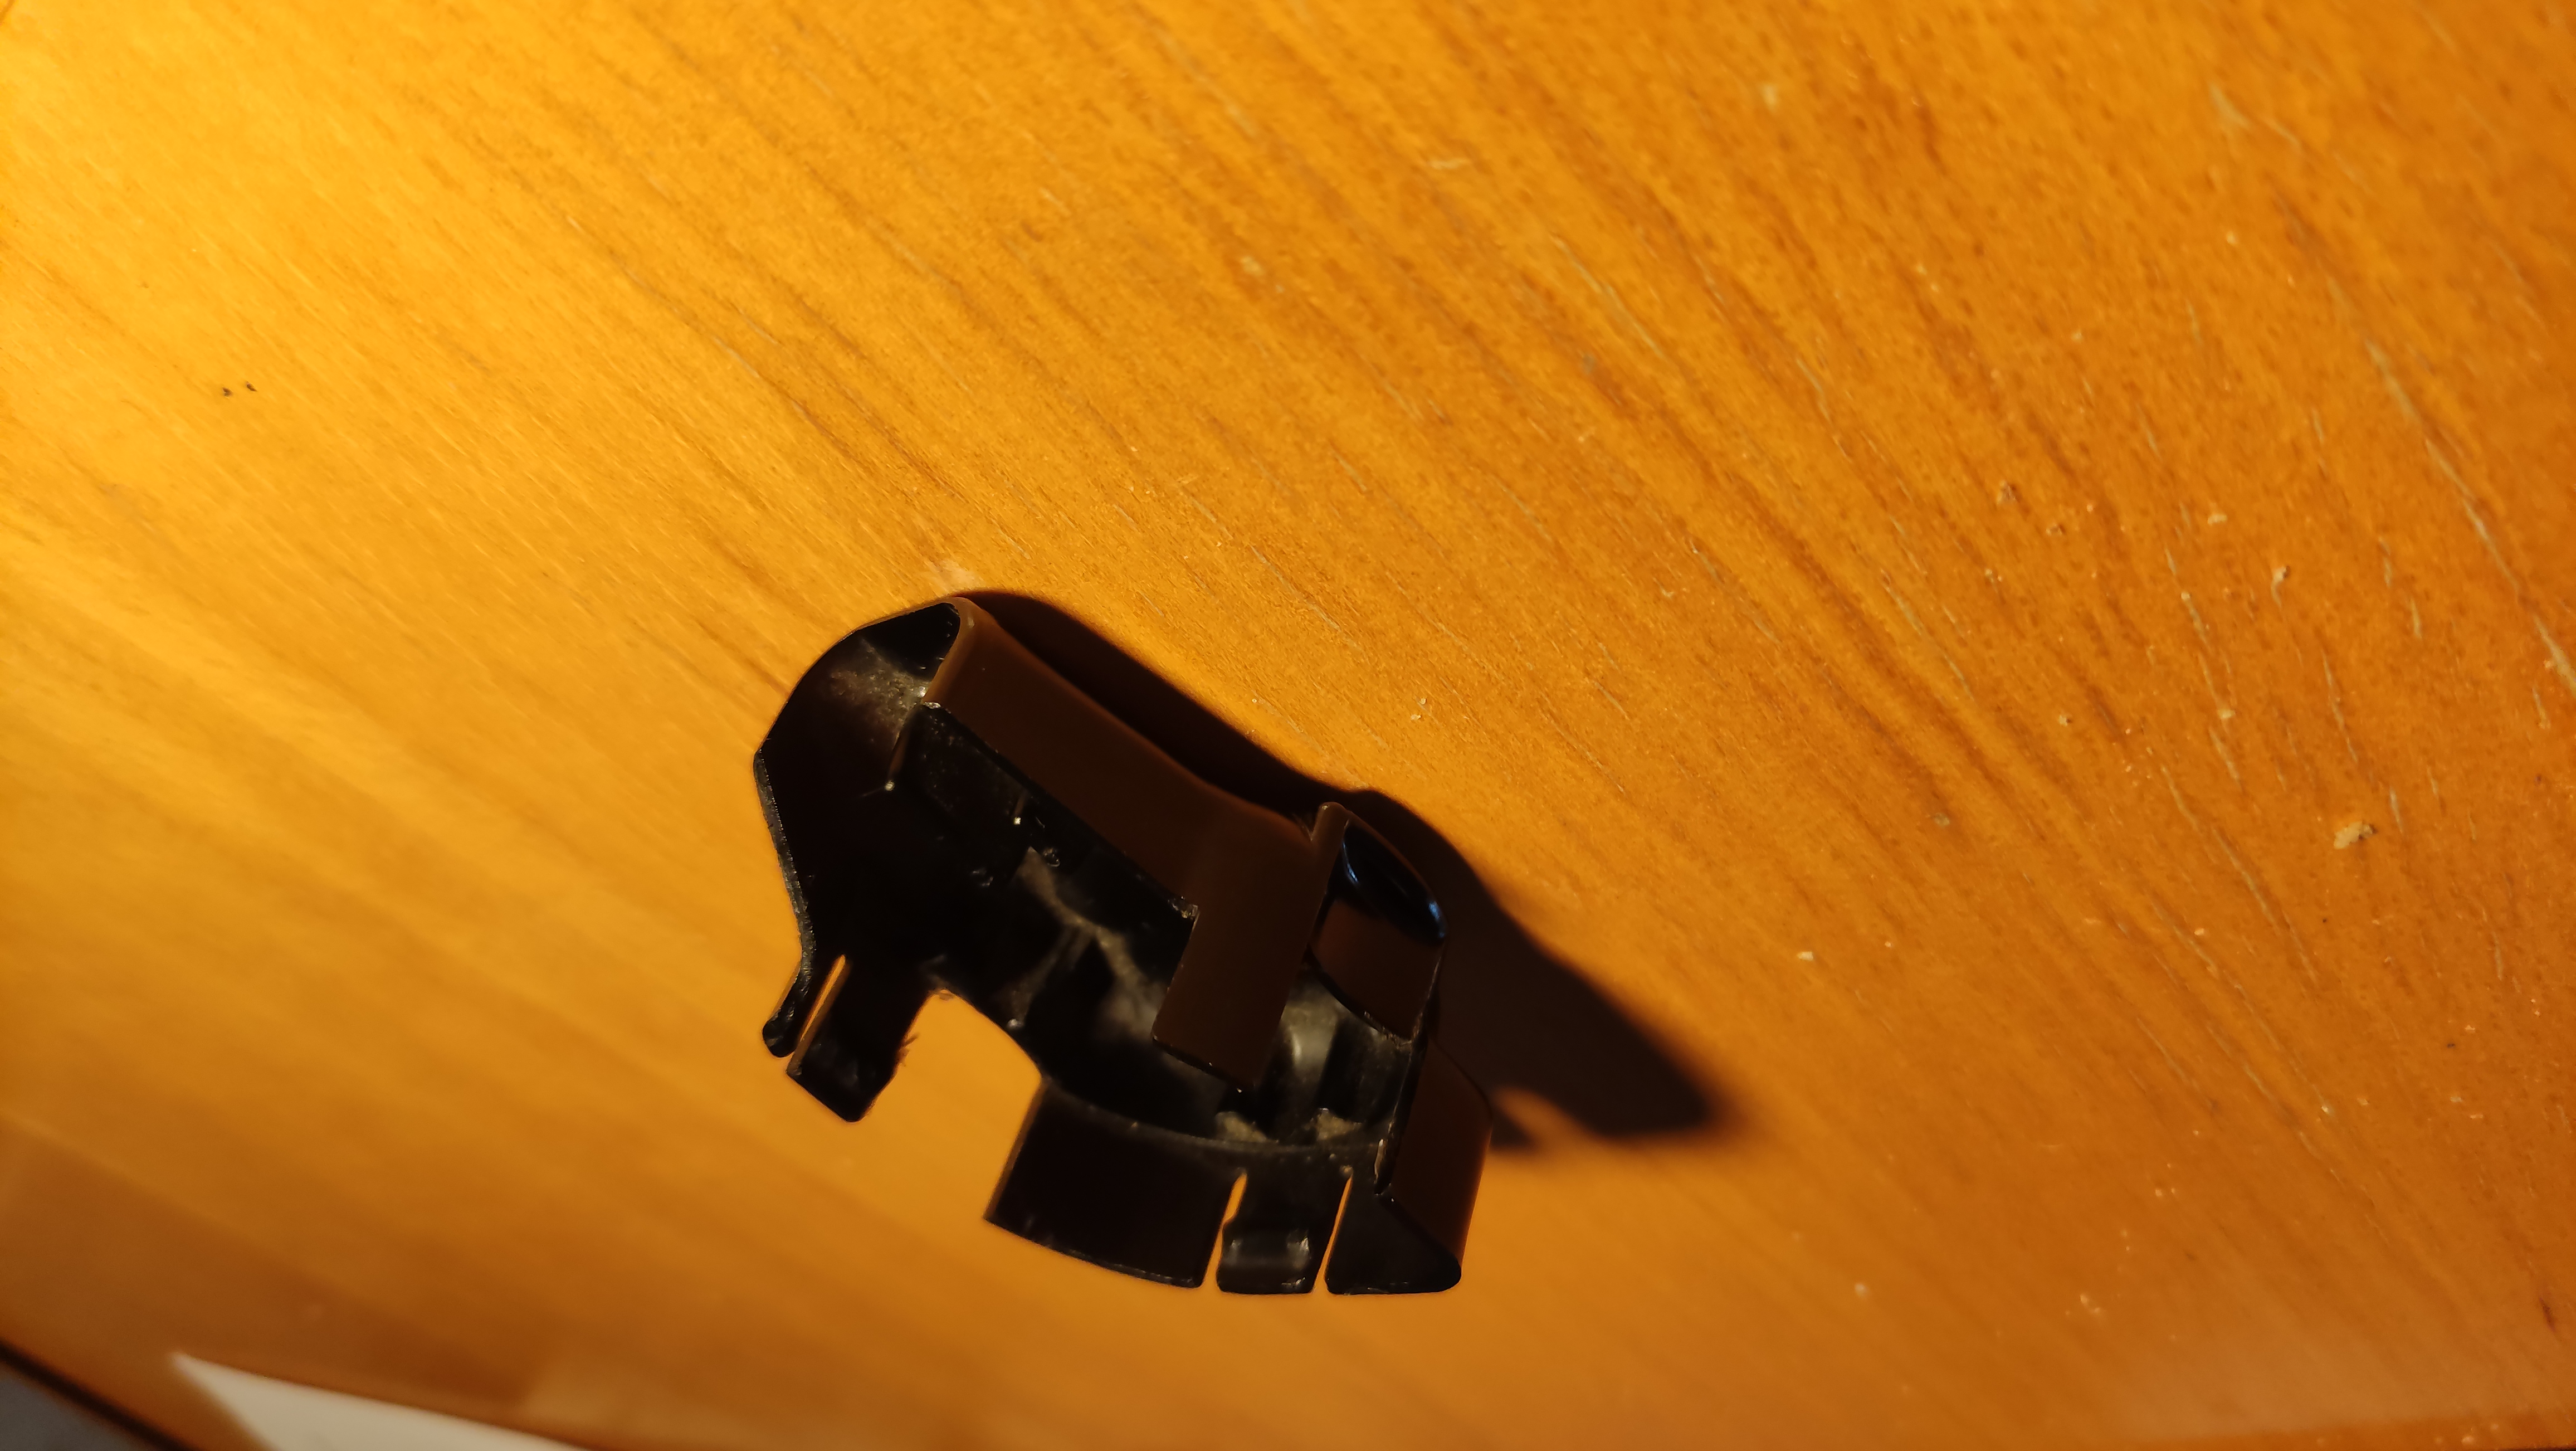
\includegraphics[width=175pt, angle=180]{img_niklas/ersatzteil2.jpg}
            \label{fig:my_label}
        \end{figure}    
    \end{minipage}
\end{figure}

\end{block}
\end{frame}

\begin{frame}{3D Scanning}
    
    \begin{minipage}[m]{.49\textwidth}
    \begin{block}{Photogrammetrie}
        \begin{itemize}
            \item \textbf{Bilder aus vielen Winkeln}
            \item Ermittlung 3D Koordinaten
            \item Point-Cloud bilden
            \item Mesh Netz spannen
            \item Rechenintensiver Prozess
            \item hohen Leistungsaufwand
            \item Qualität abhängig von Bildern
        \end{itemize}    
    \end{block}
    \end{minipage}
    \begin{minipage}[m]{.49\textwidth}
        \begin{figure}[]
          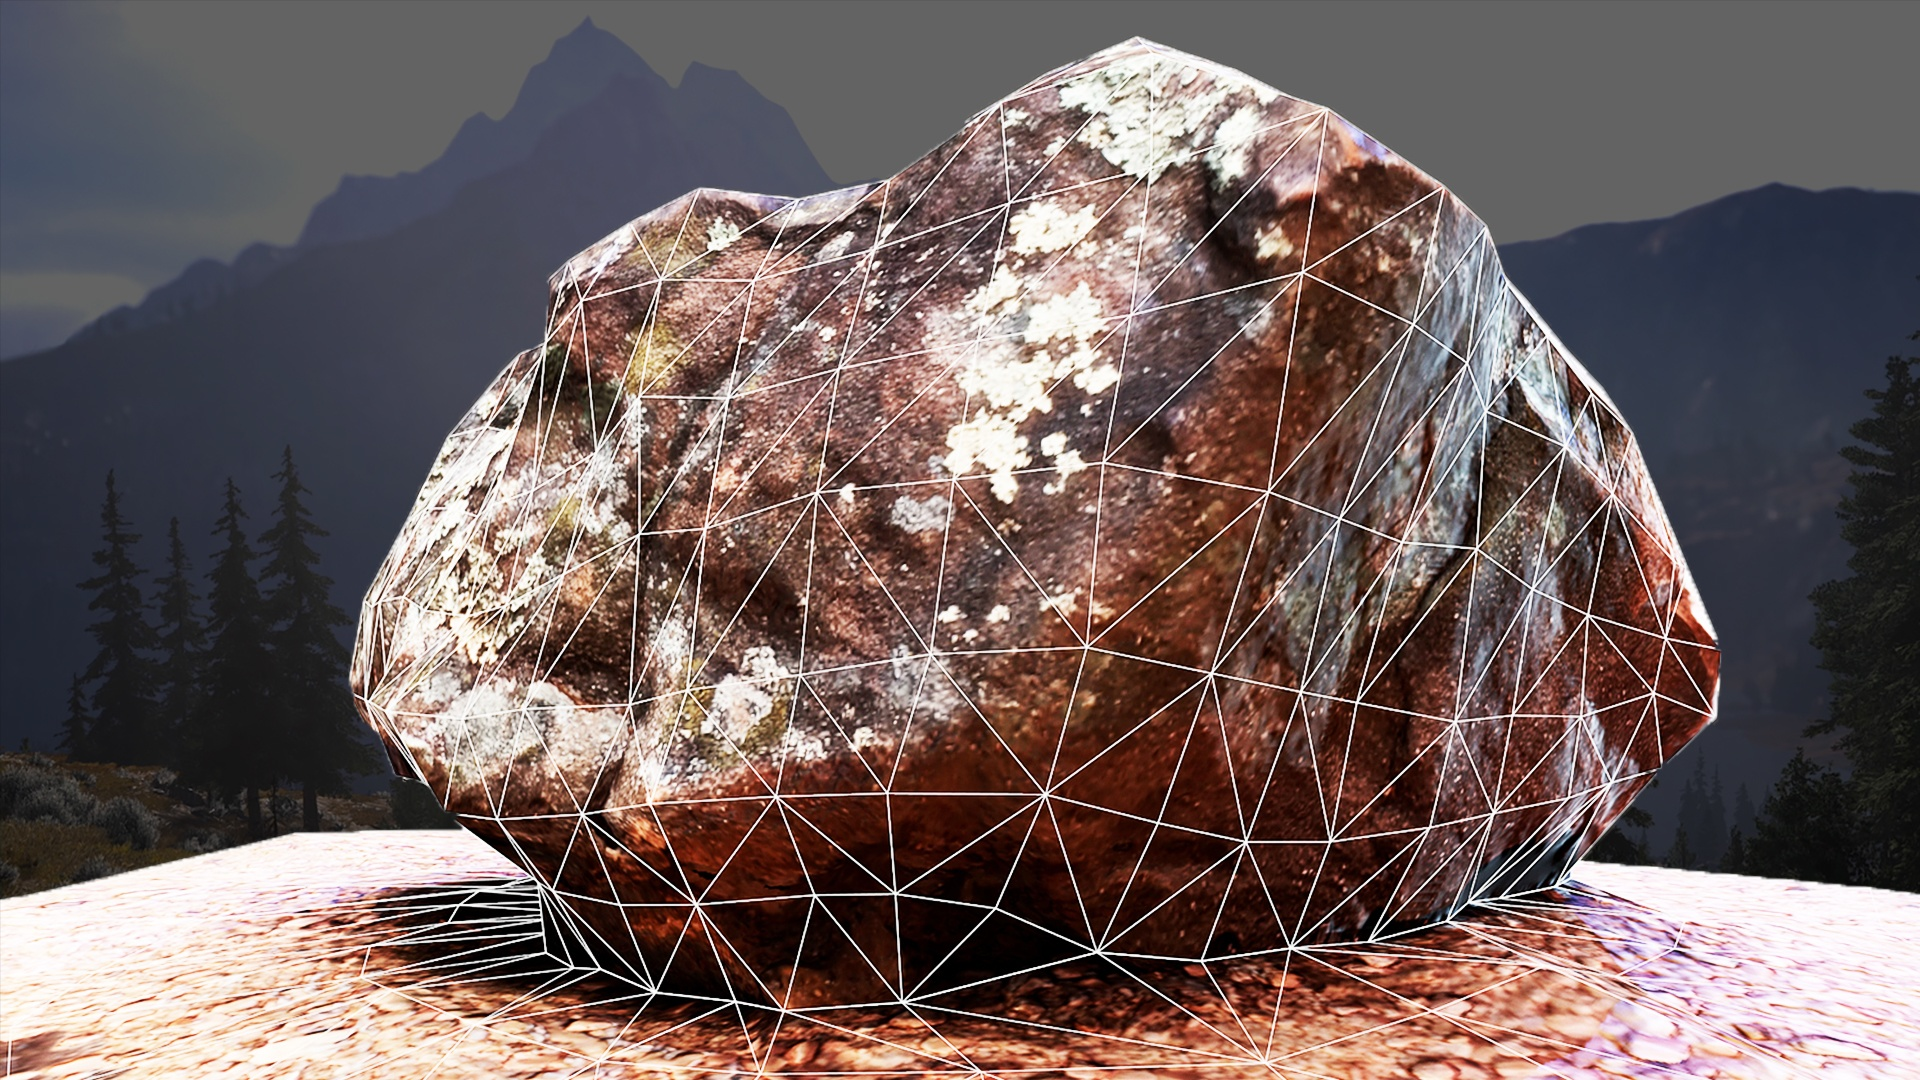
\includegraphics[width=190pt]{img_niklas/photogrammetrie_6014830.jpg}
          \label{fig:my_label}
      \end{figure}    
    \end{minipage}
    
\end{frame}

\begin{frame}{3D Scanning}
    \begin{minipage}[m]{.49\textwidth}
    \begin{block}{Photogrammetrie}
        \begin{itemize}
            \item Bilder aus vielen Winkeln
            \item \textbf{Ermittlung 3D Koordinaten}
            \item Point-Cloud bilden
            \item Mesh Netz spannen
            \item Rechenintensiver Prozess
            \item hohen Leistungsaufwand
            \item Qualität abhängig von Bildern
        \end{itemize}
        \end{block}
    \end{minipage}
    \begin{minipage}[m]{.49\textwidth}
        \begin{figure}[]
          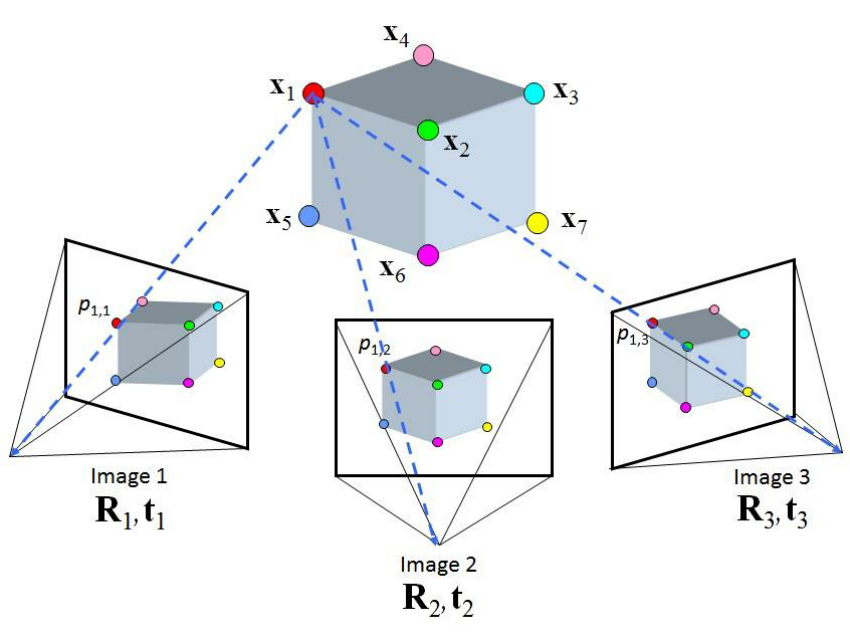
\includegraphics[height=130pt]{img_niklas/Structure-from-Motion-SfM-process-is-illustrated-The-structure-in-the.png}
          \label{fig:my_label}
      \end{figure}    
    \end{minipage}
    
\end{frame}

\begin{frame}{3D Scanning}
\begin{minipage}[m]{.49\textwidth}
    \begin{block}{Photogrammetrie}
        \begin{itemize}
            \item Bilder aus vielen Winkeln
            \item Ermittlung 3D Koordinaten
            \item \textbf{Point-Cloud bilden}
            \item Mesh Netz spannen
            \item Rechenintensiver Prozess
            \item hohen Leistungsaufwand
            \item Qualität abhängig von Bildern
        \end{itemize}  
    \end{block}
    \end{minipage}
    \begin{minipage}[]{.49\textwidth}
        \begin{figure}[]
          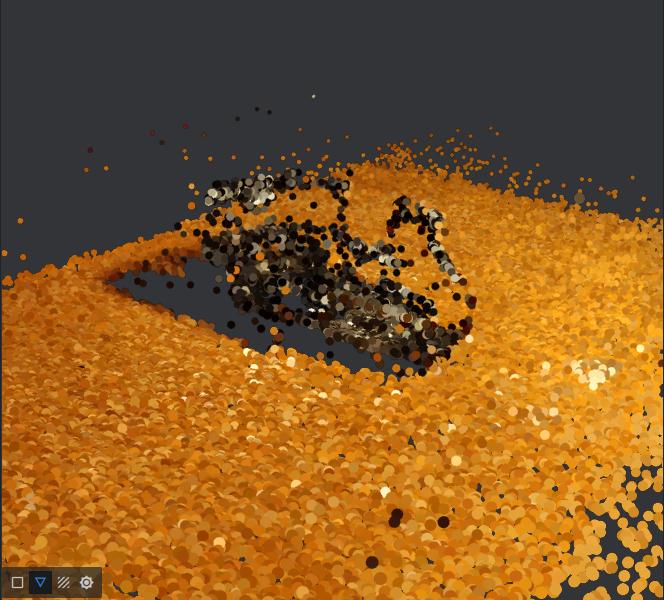
\includegraphics[height=130pt]{img_niklas/image_anlasserPointCloud.PNG}
          \label{fig:my_label}
      \end{figure}    
    \end{minipage}
    
  
\end{frame}

\begin{frame}[m]{3D Scanning}
    \begin{minipage}{.49\textwidth}
    \begin{block}{Photogrammetrie}
        \begin{itemize}
            \item Bilder aus vielen Winkeln
            \item Ermittlung 3D Koordinaten
            \item Point-Cloud bilden
            \item \textbf{Mesh Netz spannen}
            \item Rechenintensiver Prozess
            \item hohen Leistungsaufwand
            \item Qualität abhängig von Bildern
        \end{itemize}
    \end{block}
    \end{minipage}
    \begin{minipage}[m]{.49\textwidth}
        \begin{figure}[]
          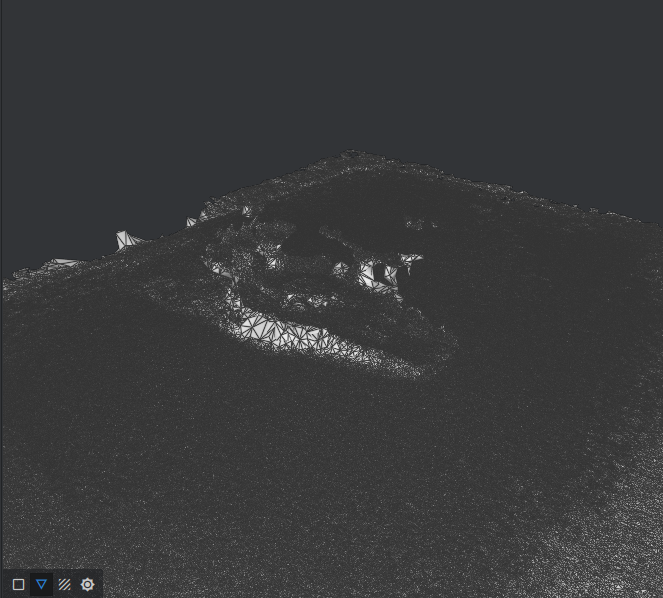
\includegraphics[height=130pt]{img_niklas/image_anlasserMesh.PNG}
          \label{fig:my_label}
      \end{figure}    
    \end{minipage}
    
\end{frame}

\begin{frame}[m]{3D Scanning}
    \begin{minipage}{.49\textwidth}
    \begin{block}{Photogrammetrie}
        \begin{itemize}
            \item Bilder aus vielen Winkeln
            \item Ermittlung 3D Koordinaten
            \item Point-Cloud bilden
            \item Mesh Netz spannen
            \item \textbf{Rechenintensiver Prozess}
            \item \textbf{hohen Leistungsaufwand}
            \item Qualität abhängig von Bildern
        \end{itemize}
    \end{block}
    \end{minipage}    
    \begin{minipage}[m]{.49\textwidth}
        \begin{figure}[]
          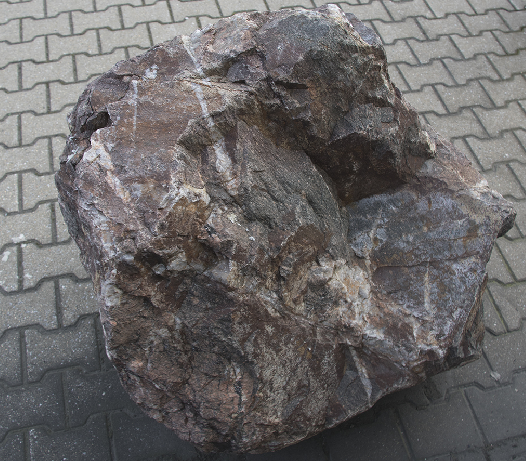
\includegraphics[height=130pt]{img_niklas/rock_image.PNG}
          \label{fig:my_label}
      \end{figure}    
    \end{minipage}
    
\end{frame}


\begin{frame}{3D Scanning}
    
    \begin{minipage}[m]{.49\textwidth}
    \begin{block}{Photogrammetrie}
        \begin{itemize}
            \item Bilder aus vielen Winkeln
            \item Ermittlung 3D Koordinaten
            \item Point-Cloud bilden
            \item Mesh Netz spannen
            \item Rechenintensiver Prozess
            \item hohen Leistungsaufwand
            \item \textbf{Qualität abhängig von Bildern}
        \end{itemize}   
    \end{block}
    \end{minipage}
    \begin{minipage}[m]{.49\textwidth}
        \begin{figure}[]
          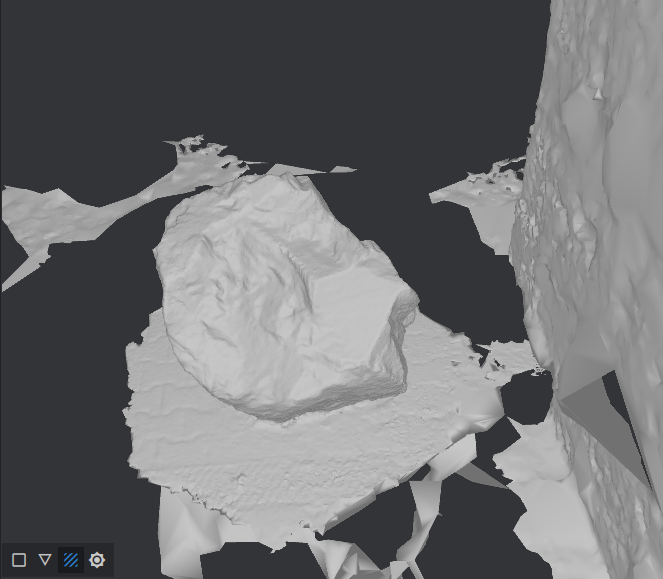
\includegraphics[height=130pt]{img_niklas/rock_3dscan.PNG}
          \label{fig:my_label}
      \end{figure}    
    \end{minipage}
    
\end{frame}

\begin{frame}{3D Scanning}
    \begin{block}{Laserscanning}
     \begin{figure}[t]
        \centering
        \begin{minipage}[m]{0.3\textwidth}
        \begin{figure}
            \centering
            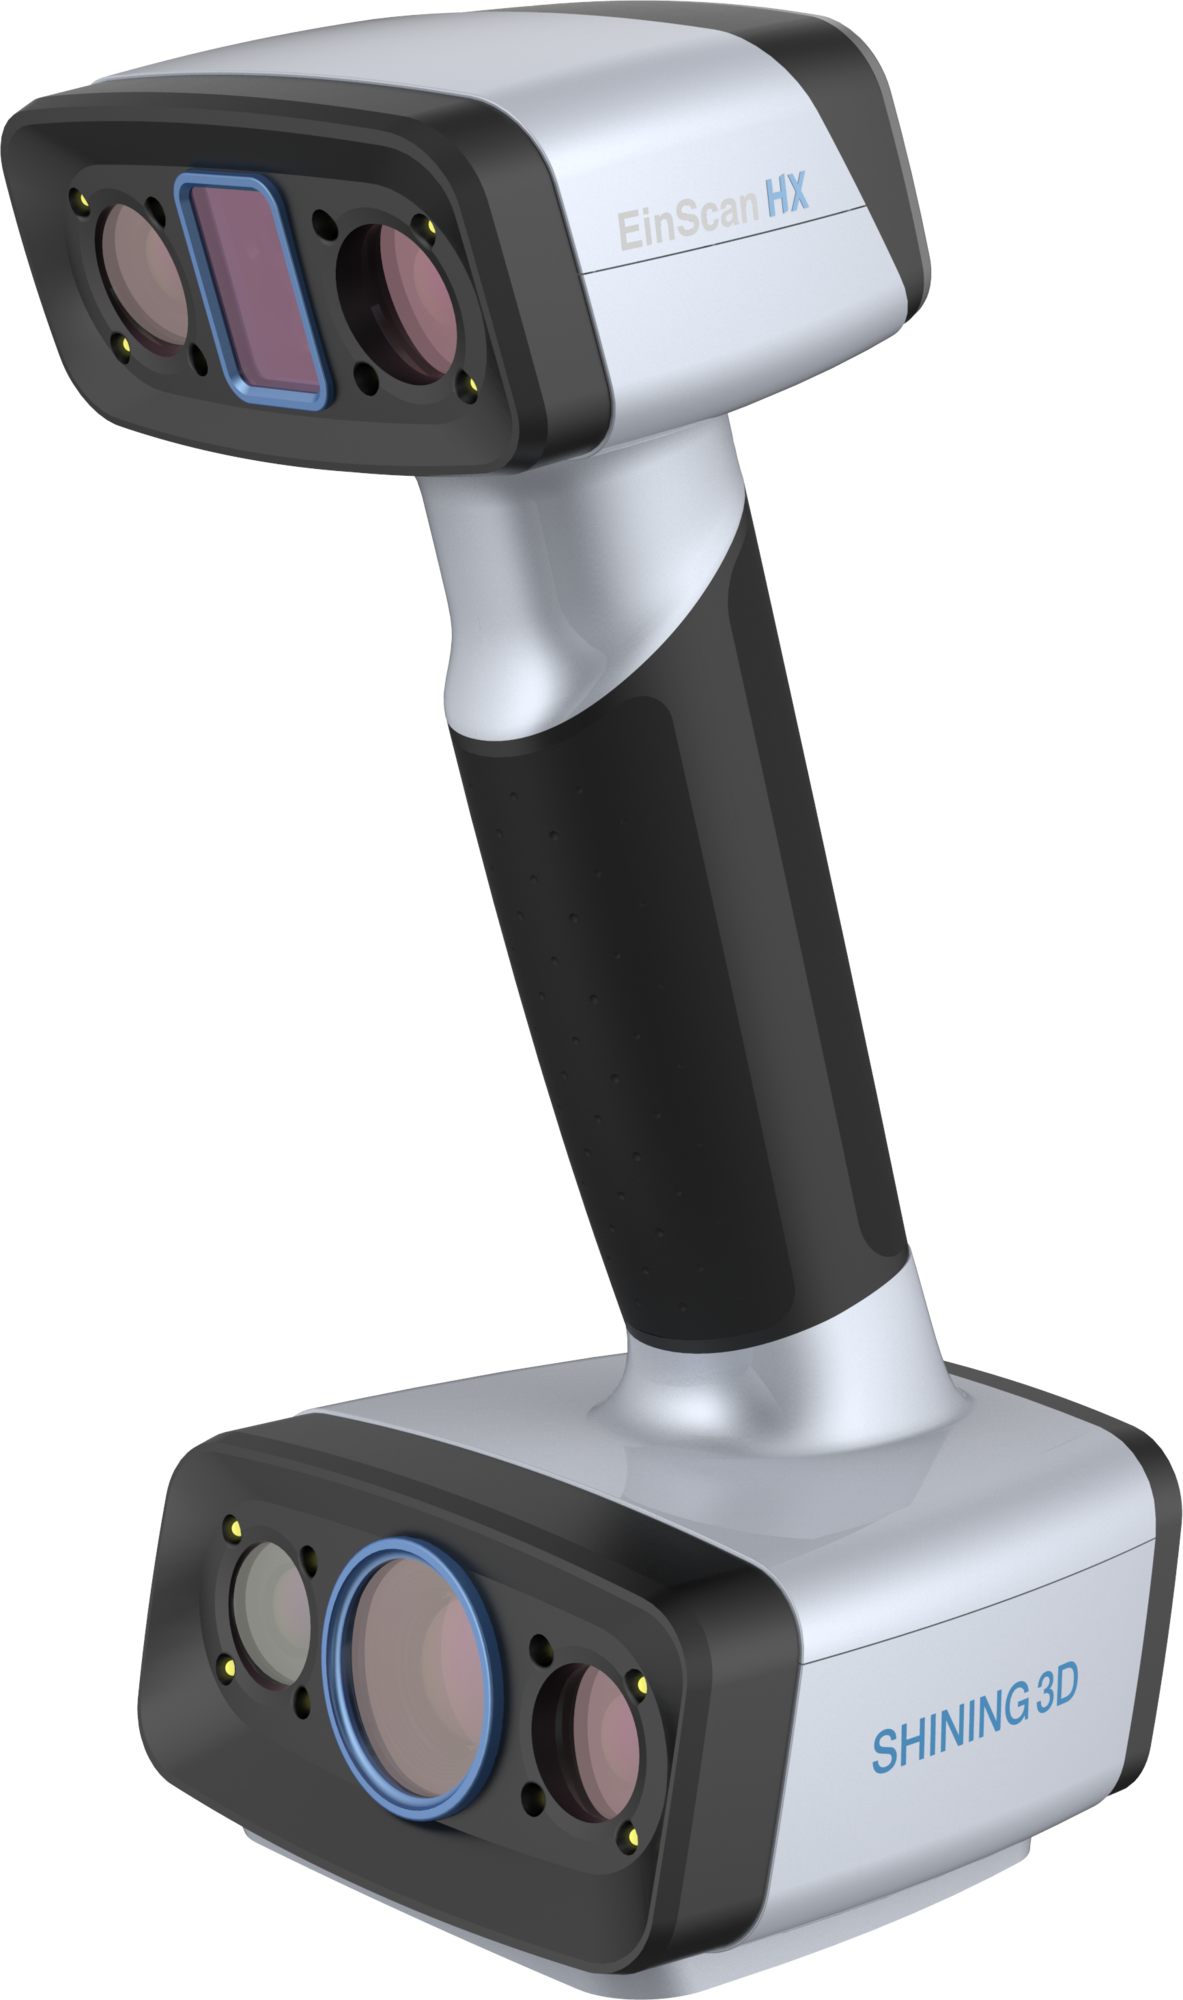
\includegraphics[height=60pt]{img_niklas/shining-3d-einscan-hx-software-bundle-solid-edge-essentials-1-stk-338985-de.png}
            \label{fig:my_label}
        \end{figure}
        \begin{figure}[b]
            \centering
            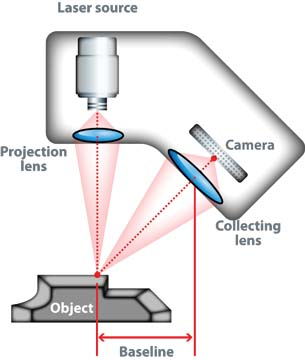
\includegraphics[height=90pt]{img_niklas/3d-scanning-101_9.jpg}
            \label{fig:my_label}
        \end{figure}
        \end{minipage}
        \hfill
        \begin{minipage}[m]{0.3\textwidth}
         \begin{figure}
            \centering
            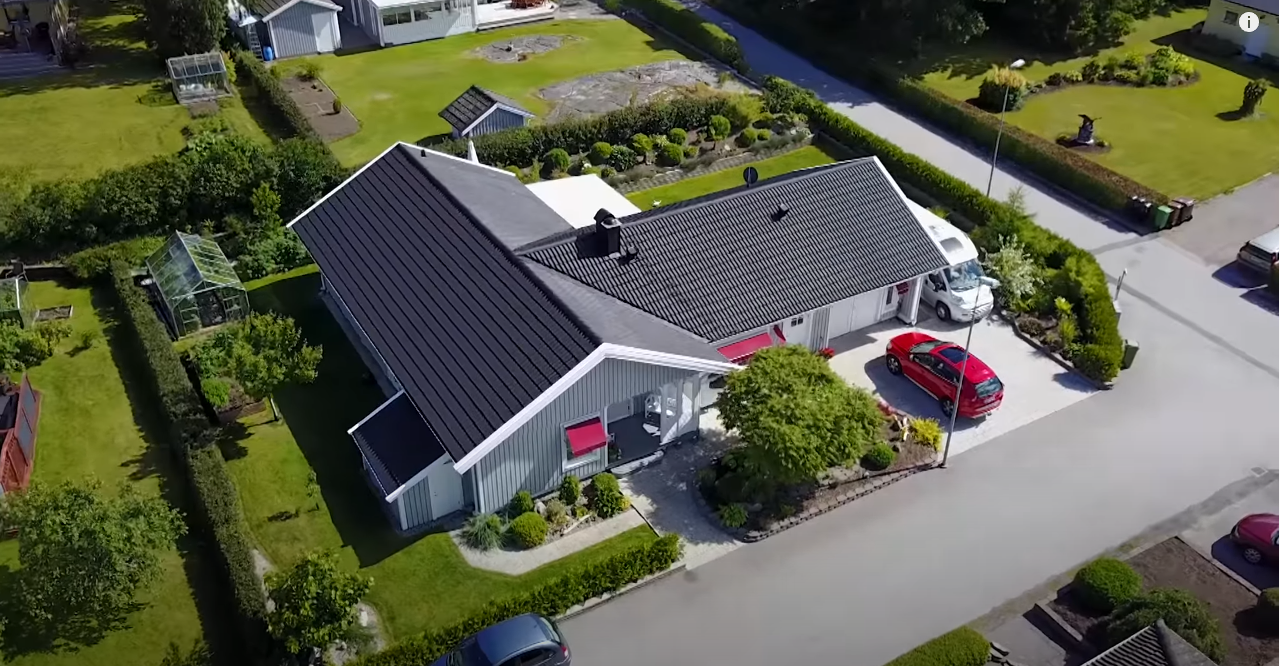
\includegraphics[height=60pt]{img_niklas/3dprintingaHouse.PNG}
            \label{fig:my_label}
        \end{figure}
        \begin{figure}[b]
            \centering
            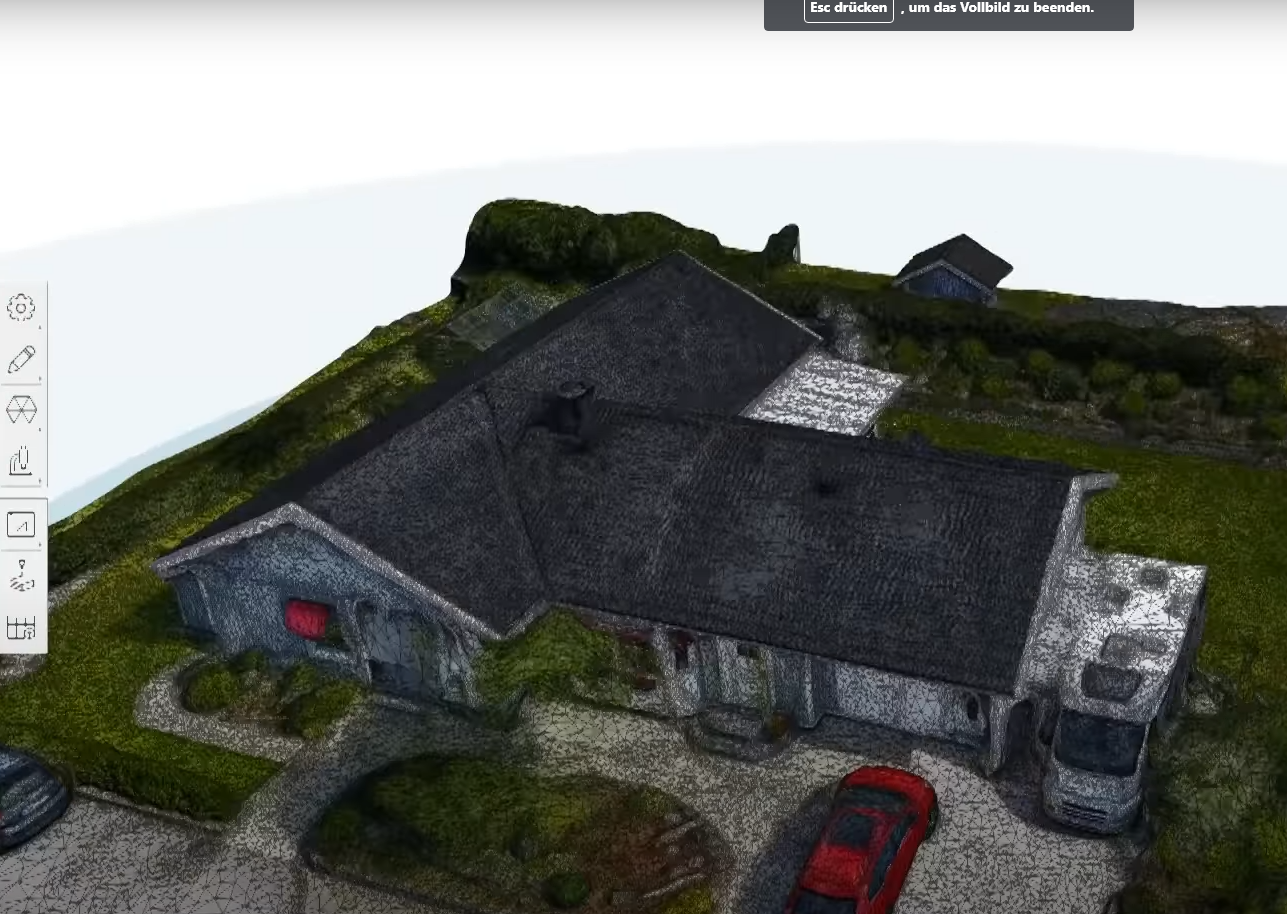
\includegraphics[height=80pt]{img_niklas/3dprintingaHouse2.PNG}
            \label{fig:my_label}
        \end{figure}
        \end{minipage}
        \hfill
        \begin{minipage}[m]{0.3\textwidth}
            \begin{itemize}
                \item Alternative zu Fotos
                \item Genaueres Ergebnis
                \item Schlechter skalierbar
                \item Teure Anschaffung
                \item Nicht immer möglich
                \item Usecase abhängig
            \end{itemize}
        \end{minipage}
    \end{figure}
    \end{block}
\end{frame}

\begin{frame}{Contact 3D scanners}
\begin{figure}
    \centering
    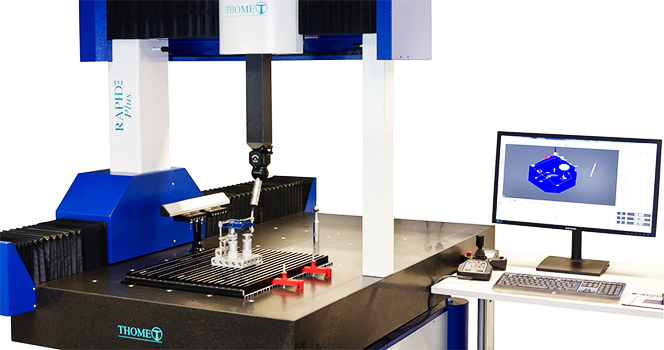
\includegraphics[width=300pt]{img_niklas/CMM.png}
    \caption*{Coordinate measuring machine}
    \label{fig:my_label}
\end{figure}
    
\end{frame}



\begin{frame}{Flugverkehr}
        \begin{figure}[t]
            \centering
            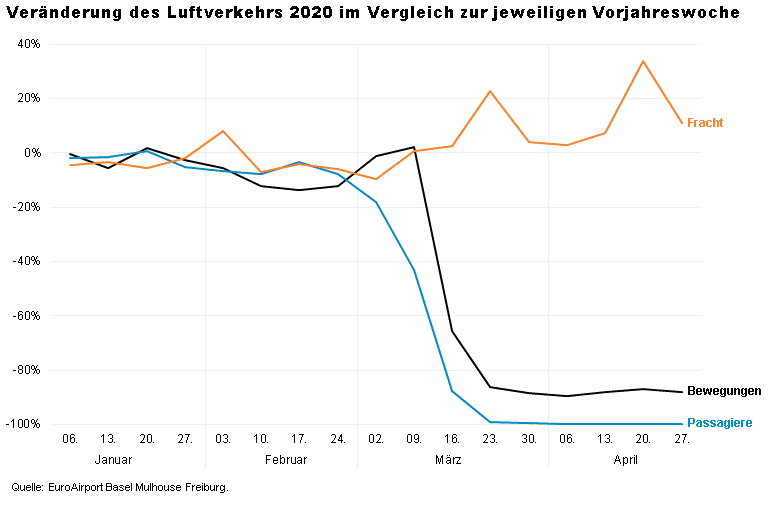
\includegraphics[height=190pt]{img_niklas/flugverkehr.PNG}
            \label{fig:my_label}
        \end{figure}
\end{frame}

\begin{frame}{CAD-Neupositionierung}
    \begin{minipage}[b]{0.7\textwidth}
    \begin{block}{Umrüstung}

    \begin{itemize}
          \item Passagierflüge durch Covid stark zurückgegangen
          \item Luftfracht ist angestiegen
          \item Boeing 777 Passagierflugzeug: 30 Tonnen Kapazität
          \item Boeing 777 Frachter: 100 Tonnen Kapazität
          \item Umrüstung von Passagierflugzeug zu Frachtmaschine
          \item Baupläne ungenau
          \item Andere Umrüstungen
      \end{itemize}
    \end{block}
    \end{minipage}
    \begin{minipage}[b]{0.27\textwidth}
        \begin{figure}
            \begin{minipage}{\textwidth}
                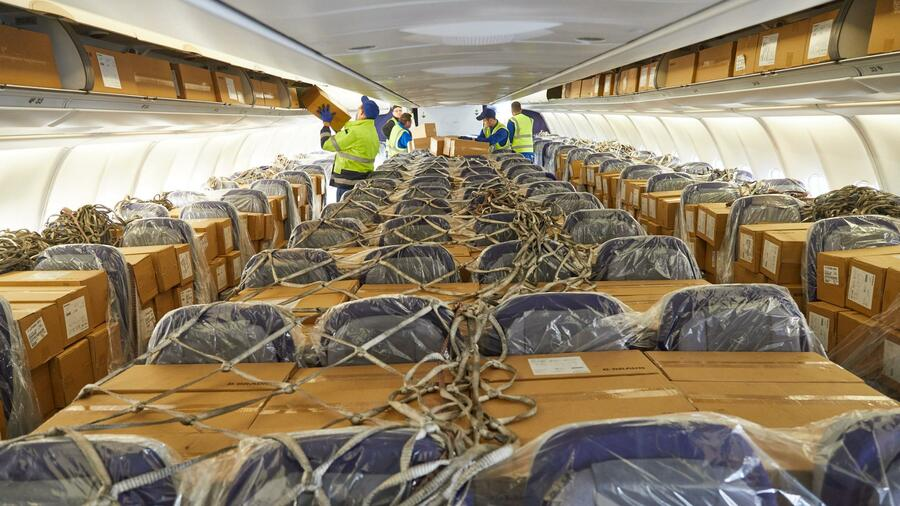
\includegraphics[width=125pt]{img_niklas/frachtMaschine.jpg}
                \label{fig:my_label}
            \end{minipage}
            \begin{minipage}{\textwidth}
                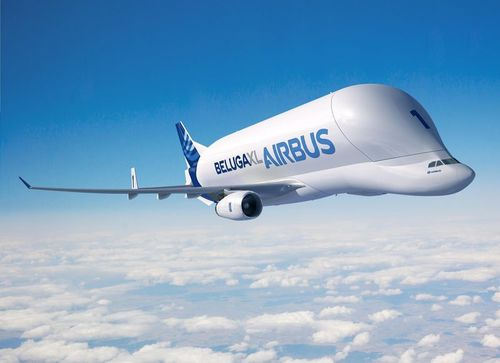
\includegraphics[width=125pt]{img_niklas/frachtFlugzeug.jpg}
            \label{fig:my_label}
            \end{minipage}
        \end{figure}
    \end{minipage}

\end{frame}

\begin{frame}{CAD-Neupositionierung}
    \begin{minipage}[]{0.5\textwidth}
    \begin{block}{Probleme}
        \begin{itemize}
            \item Baupläne oft ungenau
            \item Viele Anpassungen
            \item Großer Arbeitsaufwand
            \item Materialverschwendung
        \end{itemize}
    \end{block}
    \begin{block}{CAD-Neupositionierung}
        \begin{itemize}
            \item vorhandenes 3D Modell verbessern
            \item Genaue Planung
            \item Aufwand Minimierung
            \item Andere Nutzen
        \end{itemize}
    \end{block}
    \end{minipage}
    \begin{minipage}[]{0.49\textwidth}
      \begin{figure}
          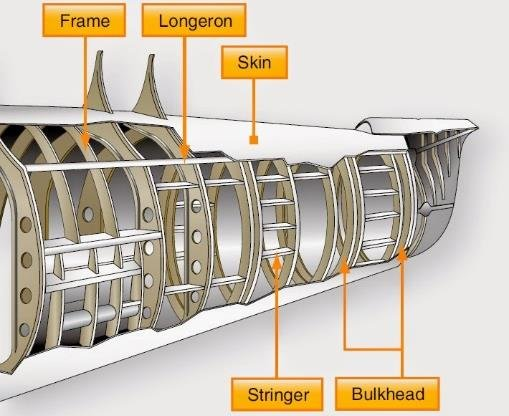
\includegraphics[width=170pt]{img_niklas/frame_Stringer.jpg}
      \end{figure}
    \end{minipage}
\end{frame}

\begin{frame}{CAD-Neupositionierung}
    \begin{minipage}[m]{0.49\textwidth}
    \begin{block}{Verfahren}
        \begin{itemize}
            \item \textbf{3D Scan und Point Cloud}
            \item Klassifizierung der Komponenten
            \item Segmentierung der Komponenten
            \item Clean up
            \item Repositionierung
            \begin{itemize}
                \item 2 Point Clouds
                \item Iterative-Closest-Point Algo.
                \item Aufsummieren des Abstands
                \item Fitness Score
            \end{itemize}
            \item Ergebnisse speichern
        \end{itemize}
    \end{block}
    \end{minipage}
    \begin{minipage}[m]{0.49\textwidth}
      \begin{figure}
          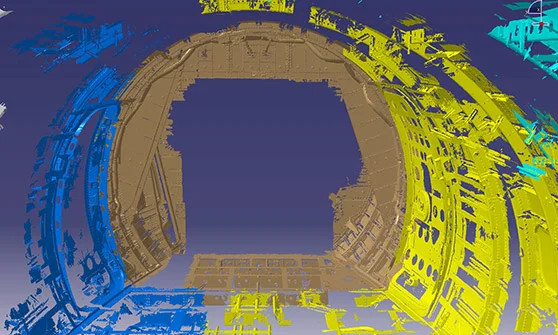
\includegraphics[width=190pt]{img_niklas/ImageForArticle_11471(1).jpg}
          \label{fig:my_label}
      \end{figure}
    \end{minipage}
\end{frame}

\begin{frame}{CAD-Neupositionierung}
    \begin{minipage}[m]{0.49\textwidth}
    \begin{block}{Verfahren}
        \begin{itemize}
            \item 3D Scan und Point Cloud
            \item \textbf{Klassifizierung der Komponenten}
            \item Segmentierung der Komponenten
            \item Clean up
            \item Repositionierung
            \begin{itemize}
                \item 2 Point Clouds
                \item Iterative-Closest-Point Algo.
                \item Aufsummieren des Abstands
                \item Fitness Score
            \end{itemize}
            \item Ergebnisse speichern
        \end{itemize}
    \end{block}
    \end{minipage}
    \begin{minipage}[m]{0.49\textwidth}
      \begin{figure}
          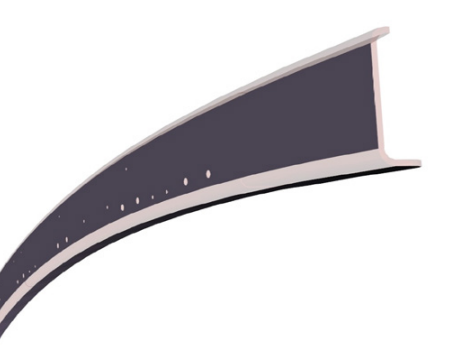
\includegraphics[width=190pt]{img_niklas/classification_frame.PNG}
          \label{fig:my_label}
      \end{figure}
    \end{minipage}
\end{frame}

\begin{frame}{CAD-Neupositionierung}
    \begin{minipage}[m]{0.49\textwidth}
    \begin{block}{Verfahren}
        \begin{itemize}
            \item 3D Scan und Point Cloud
            \item Klassifizierung der Komponenten
            \item \textbf{Segmentierung der Komponenten}
            \item Clean up
            \item Repositionierung
            \begin{itemize}
                \item 2 Point Clouds
                \item Iterative-Closest-Point Algo.
                \item Aufsummieren des Abstands
                \item Fitness Score
            \end{itemize}
            \item Ergebnisse speichern
        \end{itemize}
    \end{block}
    \end{minipage}
    \begin{minipage}[m]{0.49\textwidth}
      \begin{figure}
          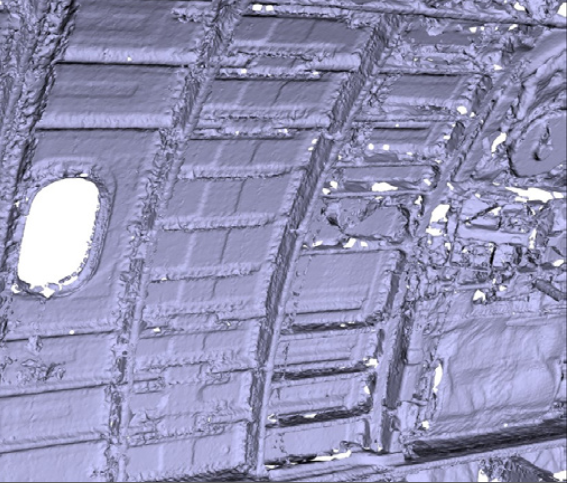
\includegraphics[width=190pt]{img_niklas/aircraft_3dscan.PNG}
          \label{fig:my_label}
      \end{figure}
    \end{minipage}
\end{frame}

\begin{frame}{CAD-Neupositionierung}
    \begin{minipage}[m]{0.49\textwidth}
    \begin{block}{Verfahren}
        \begin{itemize}
            \item 3D Scan und Point Cloud
            \item Klassifizierung der Komponenten
            \item \textbf{Segmentierung der Komponenten}
            \item Clean up
            \item Repositionierung
            \begin{itemize}
                \item 2 Point Clouds
                \item Iterative-Closest-Point Algo.
                \item Aufsummieren des Abstands
                \item Fitness Score
            \end{itemize}
            \item Ergebnisse speichern
        \end{itemize}
    \end{block}
    \end{minipage}
    \begin{minipage}[m]{0.49\textwidth}
      \begin{figure}
          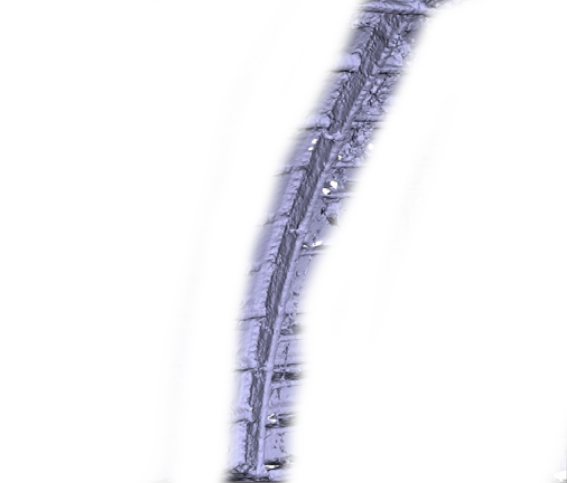
\includegraphics[width=190pt]{img_niklas/aircraft_3dscan_segmented.PNG}
          \label{fig:my_label}
      \end{figure}
    \end{minipage}
\end{frame}

\begin{frame}{CAD-Neupositionierung}
    \begin{minipage}[]{0.49\textwidth}
    \begin{block}{Verfahren}
        \begin{itemize}
            \item 3D Scan und Point Cloud
            \item Klassifizierung der Komponenten
            \item Segmentierung der Komponenten
            \item \textbf{Clean up}
            \item Repositionierung
            \begin{itemize}
                \item 2 Point Clouds
                \item Iterative-Closest-Point Algo.
                \item Aufsummieren des Abstands
                \item Fitness Score
            \end{itemize}
            \item Ergebnisse speichern
        \end{itemize}
    \end{block}
    \end{minipage}
    \begin{minipage}[]{0.49\textwidth}
      \begin{figure}
          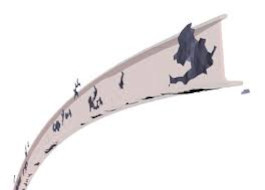
\includegraphics[width=190pt]{img_niklas/clean_up_before.jpg}
          \label{fig:my_label}
      \end{figure}
    \end{minipage}
\end{frame}

\begin{frame}{CAD-Neupositionierung}
    \begin{minipage}[]{0.49\textwidth}
    \begin{block}{Verfahren}
        \begin{itemize}
            \item 3D Scan und Point Cloud
            \item Klassifizierung der Komponenten
            \item Segmentierung der Komponenten
            \item \textbf{Clean up}
            \item Repositionierung
            \begin{itemize}
                \item 2 Point Clouds
                \item Iterative-Closest-Point Algo.
                \item Aufsummieren des Abstands
                \item Fitness Score
            \end{itemize}
            \item Ergebnisse speichern
        \end{itemize}
    \end{block}
    \end{minipage}
    \begin{minipage}[]{0.49\textwidth}
      \begin{figure}
          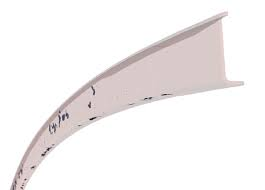
\includegraphics[width=190pt]{img_niklas/clean_up_after.jpg}
          \label{fig:my_label}
      \end{figure}
    \end{minipage}
\end{frame}


\begin{frame}{CAD-Neupositionierung}
    \begin{minipage}[]{0.49\textwidth}
    \begin{block}{Verfahren}
        \begin{itemize}
            \item 3D Scan und Point Cloud
            \item Klassifizierung der Komponenten
            \item Segmentierung der Komponenten
            \item Clean up
            \item \textbf{Repositionierung}
            \begin{itemize}
                \item 2 Point Clouds
                \item Iterative-Closest-Point Algo.
                \item Aufsummieren des Abstands
                \item Fitness Score
            \end{itemize}
            \item Ergebnisse speichern
        \end{itemize}
    \end{block}
    \end{minipage}
    \begin{minipage}[]{0.49\textwidth}
      \begin{figure}
          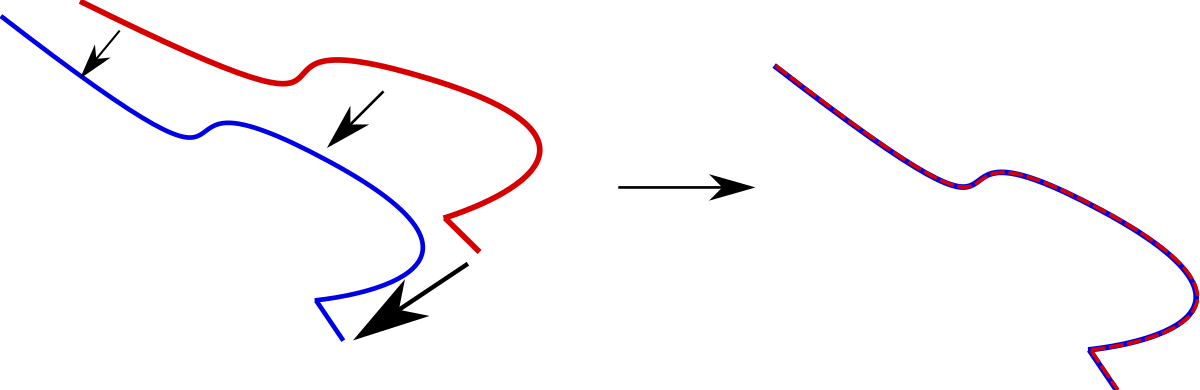
\includegraphics[width=190pt]{img_niklas/1200px-Idea_closest_point_algorithm.svg.png}
          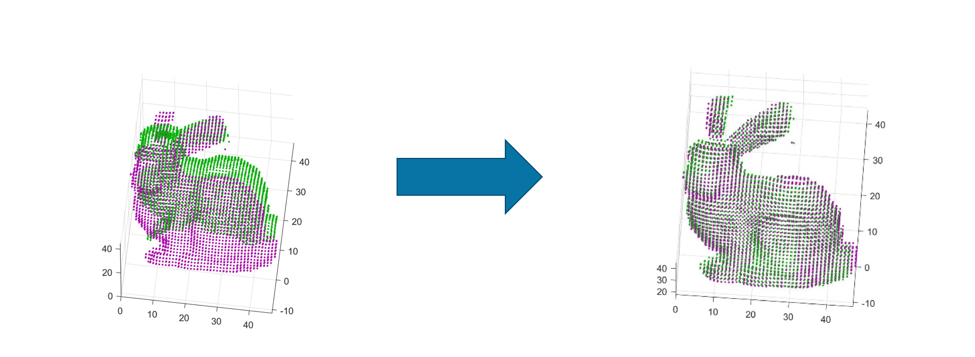
\includegraphics[width=190pt]{img_niklas/icp_3d.png}
          \label{fig:my_label}
      \end{figure}
    \end{minipage}
\end{frame}

\begin{frame}{CAD-Neupositionierung}
    \begin{minipage}[]{0.49\textwidth}
    \begin{block}{Verfahren}
        \begin{itemize}
            \item 3D Scan und Point Cloud
            \item Klassifizierung der Komponenten
            \item Segmentierung der Komponenten
            \item Clean up
            \item Repositionierung
            \begin{itemize}
                \item 2 Point Clouds
                \item Iterative-Closest-Point Algo.
                \item Aufsummieren des Abstands
                \item Fitness Score
            \end{itemize}
            \item \textbf{Ergebnisse speichern}
        \end{itemize}
    \end{block}
    \end{minipage}
    \begin{minipage}[]{0.49\textwidth}
      \begin{figure}
          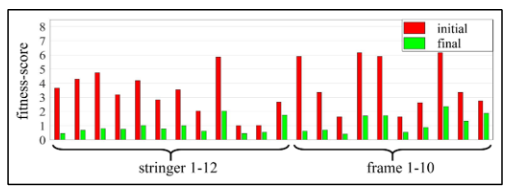
\includegraphics[width=190pt]{img_niklas/results_repo.PNG}
          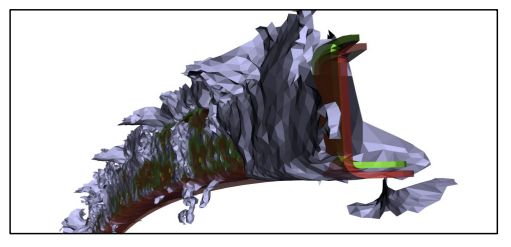
\includegraphics[width=190pt]{img_niklas/inital_vs_final.PNG}
          \label{fig:my_label}
      \end{figure}
    \end{minipage}
\end{frame}

\begin{frame}{CAD-Neupositionierung}
    \begin{block}{Zusammenfassung}
        \begin{itemize}
            \item Kombination von schon vorhandenem
            \item Open-Source
            \item Automatisierung
            \item Verbessert Modelle
            \item Minimiert Arbeitsaufwand
            \item Indikator für Modelle
        \end{itemize}
    \end{block}
\end{frame}

\begin{frame}{CAD-Neupositionierung}
\begin{figure}
    \centering
    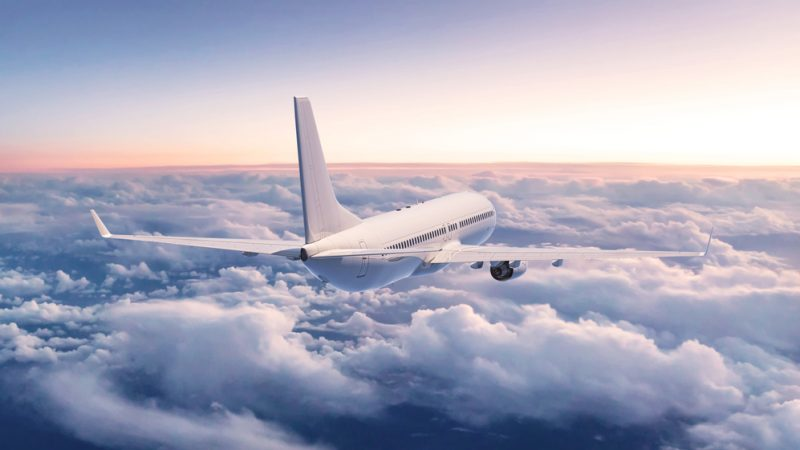
\includegraphics[height=175pt]{img_niklas/end_frame.jpg}
    \caption*{Danke fürs Zuhören}
    \label{fig:my_label}
\end{figure}

\end{frame}

\begin{frame}{Bildquellen}

\begin{minipage}[t]{0.49\textwidth}
    \small \href{https://www.thingiverse.com/thing:937740}{Low Poly Fox}\\
    \small \href{https://www.nasa.gov/mission_pages/station/research/news/3Dratchet_wrench}{ISS 3D printed wrech image}\\
    \small \href{https://nasa3d.arc.nasa.gov/detail/wrench-mis}{ISS 3D printed wrech STL}\\
    \small \href{https://www.aniwaa.com/buyers-guide/3d-printers/house-3d-printer-construction/}{3D printed house}\\
    \small \href{https://singularityhub.com/wp-content/uploads/2019/11/3d-printed-boat-3dirigo-1068x601.jpg}{3D printed boat}\\
    \small \href{https://www.coolthings.com/creality-cr-30-3dprintmill-3d-printer-conveyor-belt/}{3D printer belt}\\
    \small \href{https://3dandprint.eu/de/3d-drucker/3d-drucker-easythreed-nano/}{Classic 3D printer}\\
    \small \href{https://www.researchgate.net/figure/Schematic-of-an-FDM-3D-printer-Reproduced-with-permission-from-12_fig1_292985550}{FDM Diagramm}\\
    \small \href{https://www.amazon.de/Creality-Motherboard-Meanwell-Carborundum-220x220x250mm/dp/B07FFTHMMN}{FDM 3D printer}\\
    \small \href{https://www.3dnatives.com/de/stereolithografie/}{SLA 3D printer}\\
    \small \href{https://3druck.com/glossar/sla/}{SLA Diagramm}\\
    \small \href{https://additivemanufacturingindia.blogspot.com/2018/04/cad-conversion-and-stl-file-in-additive.html}{STL Resolution}\\
    \small VW T1 und Ersatzteil [Eigene Bilder]\\
    \small \href{https://www.gamestar.de/videos/photogrammetrie-wie-macht-man-spiele-photorealistisch,94973.html}{Photogrammetrie Netz}\\
    \small \href{https://www.researchgate.net/figure/Structure-from-Motion-SfM-process-is-illustrated-The-structure-in-the_fig2_269327935}{Photogrammetrie Kameras}\\
    \small Ersatzteil Point Cloud und Mesh [Eigene Bilder]\\
\end{minipage}
\begin{minipage}[t]{0.49\textwidth}
    \small \href{https://www.turbosquid.com/de/3d-models/3d-photogrammetry-scan-stone-08-model-1321356}{Photogrammetrie Stein}\\
    \small \href{https://www.3djake.de/shining-3d/einscan-hx}{Handheld laser scanner}\\
    \small \href{https://3dscanningservices.net/blog/what-you-need-to-know-about-3d-scanning/}{Laserscanning Funktionsweise}\\
    \small \href{https://www.youtube.com/watch?v=YiPBpgF000g}{3D Scan of House}\\
    \small \href{https://www.thome-precision.com/images/Messmaschine/CMM.png}{Contact 3D Scanner}\\
    \small \href{https://www.statistik.bs.ch/themenspeicher/eap-luftverkehr.html}{Fluverkehr Statistik}\\
    \small \href{https://www.aeroexpo.online/de/prod/airbus/product-173753-382.html}{Airbus Frachtflugzeug}\\
    \small \href{https://www.handelsblatt.com/unternehmen/handel-konsumgueter/lufthansa-cargo-die-luftfracht-boomt-und-setzt-auch-auf-leere-passagierjets-/25695540.html}{Passiermaschine Fracht}\\
    \small \href{https://www.researchgate.net/figure/Stringer-location-on-aircraft-fuselage_fig1_325518126}{Frame and Stringer}\\
    \small \href{https://www.creaform3d.com/blog/de/erfolgsgeschichten/engineering-eines-flugzeuginnenraums-vom-scan-zum-3d-modell/}{Airplane 3D Scan}\\
    \small \href{https://www.sciencedirect.com/science/article/pii/S2212827121005874?ref=pdf_download&fr=RR-2&rr=7252baca68ce7162}{Folie 22 - 25}\\
    \small \href{https://de.wikipedia.org/wiki/Iterative_Closest_Point_Algorithm}{ICP Algo.}\\
    \small \href{https://hanzhoulu.github.io/Parallel-Point-Cloud-Registration/}{ICP Point Clouds}\\
    \small \href{https://www.sciencedirect.com/science/article/pii/S2212827121005874?ref=pdf_download&fr=RR-2&rr=7252baca68ce7162}{Folie 27}\\
    \small \href{https://www.euractiv.de/section/biokraftstoffe/news/eu-kommission-schlaegt-instrumente-fuer-nachhaltige-flugzeug-kraftstoffe-vor/}{Ende Flugzeug}\\
    \end{minipage}
\end{frame}



\end{document} 
